% =============================================================================
% SECCION: RESULTADOS EMPIRICOS (EXPANDIDA)
% =============================================================================

\section{Resultados Emp\'iricos}
\label{sec:empirical_results}

En esta secci\'on se presentan los resultados del \hyperlink{glos:backtesting}{\textit{backtesting}} de los 23 modelos durante el per\'iodo de prueba (octubre 2020 a diciembre 2025, 1{,}302 d\'ias de \textit{trading}).

\subsection{Rendimiento General}
\label{subsec:performance_summary}

La Tabla~\ref{tab:model_performance} presenta las m\'etricas de rendimiento completas para los 23 modelos evaluados.

\begin{table}[htbp]
\centering
\caption{Rendimiento de los 23 Modelos en el Per\'iodo de Prueba (Oct 2020 - Dic 2025)}
\label{tab:model_performance}
\small
\begin{tabular}{@{}llrrrrr@{}}
\toprule
\textbf{Rank} & \textbf{Modelo} & \textbf{Categor\'ia} & \textbf{Ret. Total} & \textbf{Ret. Anual} & \textbf{Sharpe} & \textbf{Max DD} \\
\midrule
1 & \textbf{LSTM\_Attention} & Deep learning & \textcolor{ForestGreen}{395.4\%} & 36.3\% & 1.319 & 20.5\% \\
2 & \textbf{Ridge} & ML cl\'asico & \textcolor{ForestGreen}{252.5\%} & 27.6\% & 0.856 & 31.8\% \\
3 & \textbf{RandomForest} & ML cl\'asico & \textcolor{ForestGreen}{127.5\%} & 17.3\% & 0.651 & 15.0\% \\
4 & \textbf{CNN\_LSTM} & Deep learning & \textcolor{ForestGreen}{122.2\%} & 16.7\% & 0.572 & 35.9\% \\
5 & DLinear & Deep learning & \textcolor{ForestGreen}{67.7\%} & 10.5\% & 0.425 & 33.4\% \\
6 & GradientBoosting & Boosting & \textcolor{ForestGreen}{66.3\%} & 10.4\% & 0.617 & 8.3\% \\
7 & CatBoost & Boosting & \textcolor{ForestGreen}{46.0\%} & 7.6\% & 0.221 & 31.4\% \\
8 & Theta & Series temporales & \textcolor{ForestGreen}{44.4\%} & 7.4\% & 0.560 & 12.6\% \\
9 & NBEATS & Deep learning & \textcolor{ForestGreen}{43.9\%} & 7.3\% & 0.178 & 25.2\% \\
\rowcolor{naivebg} 10 & SeasonalNaive$^\dagger$ & Series temporales & \textcolor{ForestGreen}{43.0\%} & 7.2\% & 0.142 & 33.6\% \\
11 & Lasso & ML cl\'asico & \textcolor{ForestGreen}{37.7\%} & 6.4\% & 0.190 & 19.5\% \\
12 & GARCH & Series temporales & \textcolor{ForestGreen}{26.6\%} & 4.7\% & 0.188 & 22.1\% \\
13 & LightGBM & Boosting & \textcolor{ForestGreen}{25.5\%} & 4.5\% & 0.088 & 24.4\% \\
14 & NHiTS & Deep learning & \textcolor{ForestGreen}{21.4\%} & 3.8\% & 0.031 & 48.3\% \\
15 & AutoARIMA$^\ddagger$ & Series temporales & \textcolor{ForestGreen}{18.3\%} & 3.3\% & 0.387 & 0.0\% \\
16 & TCN & Deep learning & \textcolor{ForestGreen}{18.0\%} & 3.3\% & 0.000 & 35.0\% \\
17 & TFT & Deep learning & \textcolor{ForestGreen}{13.5\%} & 2.5\% & -0.028 & 45.2\% \\
18 & Prophet & Series temporales & \textcolor{ForestGreen}{7.8\%} & 1.5\% & -0.230 & 11.7\% \\
19 & ElasticNet & ML cl\'asico & \textcolor{ForestGreen}{7.8\%} & 1.5\% & -0.085 & 40.4\% \\
20 & XGBoost & Boosting & \textcolor{ForestGreen}{7.1\%} & 1.3\% & -0.060 & 45.7\% \\
21 & BiLSTM & Deep learning & \textcolor{ForestGreen}{4.9\%} & 0.9\% & -0.091 & 55.1\% \\
22 & ExponentialSmoothing & Series temporales & \textcolor{BrickRed}{-15.4\%} & -3.2\% & -0.241 & 60.3\% \\
23 & BiGRU & Deep learning & \textcolor{BrickRed}{-33.2\%} & -7.5\% & -0.467 & 59.0\% \\
\midrule
-- & SPY (B\&H) & Benchmark & 101.3\% & -- & 0.657 & 25.4\% \\
\bottomrule
\end{tabular}
\begin{tablenotes}
\small
\item Nota: Los modelos en negrita superan al benchmark SPY Buy \& Hold. \colorbox{naivebg}{$^\dagger$SeasonalNaive} = \textit{benchmark} de complejidad m\'inima. $^\ddagger$AutoARIMA permanece el 100\% del per\'iodo en efectivo (filtro de calidad de se\~nal), por lo que su retorno corresponde a la tasa libre de riesgo y su Sharpe, calculado sobre una volatilidad casi nula (0.14\%), no es comparable con el de los modelos con operaci\'on activa. Retorno total calculado como producto de (1+r) - 1 sobre el per\'iodo completo. Sharpe ratio anualizado con tasa libre de riesgo promedio del per\'iodo.
\end{tablenotes}
\end{table}


Cuatro de veintitr\'es modelos superan al \textit{benchmark} SPY Buy \& Hold (+101.3\%), a saber, LSTM+Attention (+395\%), Ridge (+253\%), RandomForest (+128\%) y CNN-LSTM (+122\%). La arquitectura con mecanismo de atenci\'on (LSTM+Attention) obtiene el mejor rendimiento tanto en t\'erminos absolutos como ajustados por riesgo, mientras que la arquitectura h\'ibrida convolucional-recurrente (CNN-LSTM) tambi\'en supera al \textit{benchmark}, si bien con un retorno inferior, lo que sugiere que estas arquitecturas capturan dependencias temporales en los retornos del S\&P~500 que los modelos m\'as simples no logran explotar.

La variabilidad entre modelos es significativa, dado que los retornos totales abarcan un rango de 429 puntos porcentuales, desde el +395\% de LSTM+Attention hasta el $-$33\% de BiGRU. No obstante, 16 de 23 modelos logran un \hyperlink{glos:sharpe_ratio}{\textit{Sharpe ratio}} positivo, lo que indica retornos ajustados por riesgo positivos en la mayor\'ia de los casos, aunque solo cuatro alcanzan el alfa necesario para superar al \textit{benchmark} pasivo.

La Tabla~\ref{tab:executive_summary} sintetiza las m\'etricas principales de los cuatro modelos ganadores frente a los \textit{benchmarks}.

\begin{table}[htbp]
\centering
\caption{Resumen Ejecutivo: Top 5 Modelos vs Benchmark}
\label{tab:executive_summary}
\begin{tabular}{@{}lrrrrr@{}}
\toprule
\textbf{Modelo} & \textbf{Ret. Total} & \textbf{Sharpe} & \textbf{Max DD} & \textbf{Capital Final} & \textbf{$\alpha$ vs SPY} \\
\midrule
LSTM\_Attention & \textbf{\textcolor{ForestGreen}{395.4\%}} & 1.319 & 20.5\% & \$49,538 & \textcolor{ForestGreen}{294.1\%} \\
Ridge & \textbf{\textcolor{ForestGreen}{252.5\%}} & 0.856 & 31.8\% & \$35,254 & \textcolor{ForestGreen}{151.2\%} \\
RandomForest & \textbf{\textcolor{ForestGreen}{127.5\%}} & 0.651 & 15.0\% & \$22,749 & \textcolor{ForestGreen}{26.2\%} \\
CNN\_LSTM & \textbf{\textcolor{ForestGreen}{122.2\%}} & 0.572 & 35.9\% & \$22,222 & \textcolor{ForestGreen}{20.9\%} \\
DLinear & 67.7\% & 0.425 & 33.4\% & \$16,771 & -33.6\% \\
\midrule
SPY (B\&H) & 101.3\% & 0.657 & 25.4\% & \$20,131 & -- \\
\bottomrule
\end{tabular}
\begin{tablenotes}
\small
\item Nota: Per\'iodo de prueba: Oct 2020 a Dic 2025 (1,302 d\'ias). Capital inicial: \$10,000. $\alpha$ = exceso de retorno sobre SPY Buy \& Hold.
\end{tablenotes}
\end{table}


\subsection{An\'alisis por Familia de Modelos}
\label{subsec:family_analysis}

La Tabla~\ref{tab:category_comparison} agrupa los 23 modelos por familia metodol\'ogica.

\begin{table}[htbp]
\centering
\caption{Rendimiento Promedio por Categor\'ia de Modelo}
\label{tab:category_comparison}
\begin{tabular}{@{}lrrrrr@{}}
\toprule
\textbf{Categor\'ia} & \textbf{N} & \textbf{Ret. Prom.} & \textbf{Mejor Ret.} & \textbf{Sharpe Prom.} & \textbf{Mejor Modelo} \\
\midrule
ML cl\'asico & 4 & \textcolor{ForestGreen}{106.4\%} & 252.5\% & 0.403 & Ridge \\
Deep learning & 9 & \textcolor{ForestGreen}{72.6\%} & 395.4\% & 0.215 & LSTM\_Attention \\
Boosting & 4 & \textcolor{ForestGreen}{36.2\%} & 66.3\% & 0.217 & GradientBoosting \\
Series temporales & 6 & \textcolor{ForestGreen}{20.8\%} & 44.4\% & 0.134 & Theta \\
\bottomrule
\end{tabular}
\begin{tablenotes}
\small
\item Nota: N = n\'umero de modelos en la categor\'ia. ML cl\'asico = Ridge/Lasso/ElasticNet/RandomForest; Boosting = GradientBoosting (sklearn) y las librer\'ias XGBoost/LightGBM/CatBoost; Series temporales = AutoARIMA/ETS/Theta/SeasonalNaive/Prophet/GARCH; Deep learning = redes Darts (DLinear/N-BEATS/N-HiTS/TCN/TFT) y arquitecturas \textit{custom} en PyTorch (CNN-LSTM/LSTM+Attention/BiLSTM/BiGRU).
\end{tablenotes}
\end{table}


Dentro del \textbf{ML cl\'asico}, Ridge destaca con un retorno del +253\% y un Sharpe de 0.86, posicion\'andose como el segundo mejor modelo del estudio, y RandomForest (+128\%, Sharpe 0.65) constituye el otro integrante de esta familia que supera al \textit{benchmark}, ambos analizados con mayor detalle en las secciones de gesti\'on de riesgo y validaci\'on estad\'istica. Lasso (+38\%) y ElasticNet (+8\%), en cambio, presentan un rendimiento marcadamente inferior, lo que sugiere que la regularizaci\'on $L_1$, que fuerza coeficientes a cero, resulta demasiado agresiva para este problema, eliminando predictores que contienen se\~nal \'util. La penalizaci\'on $L_2$ de Ridge, que contrae los coeficientes sin eliminarlos, se adapta mejor a un espacio de 536 caracter\'isticas donde la se\~nal est\'a distribuida entre m\'ultiples predictores.

En la categor\'ia de \textbf{\textit{boosting}}, GradientBoosting lidera con un retorno del +66\% y un Sharpe de 0.62, destac\'andose adem\'as por el menor \hyperlink{glos:drawdown}{\textit{drawdown}} m\'aximo de todo el estudio entre los modelos con operaci\'on activa (8.3\%), si bien la baja variabilidad de sus predicciones (apenas 16 valores \'unicos) lo mantiene filtrado en efectivo el 86\% del tiempo. Le siguen CatBoost (+46\%, Sharpe 0.22), LightGBM (+25\%) y XGBoost (+7\%). Ninguno de los cuatro supera al \textit{benchmark}, lo que indica que los umbrales din\'amicos del Meta-KNN resultan menos efectivos para estos modelos basados en \'arboles cuando sus predicciones presentan baja variabilidad, dado que XGBoost, por ejemplo, genera apenas 26 valores \'unicos y permanece filtrado el 62\% del tiempo, lo que degrada la calidad de la se\~nal de posicionamiento.

Los modelos de \textbf{\textit{deep learning} implementados en Darts} exhiben un rendimiento inferior al esperado dada su complejidad arquitectural. DLinear obtiene el mejor resultado de la subcategor\'ia con +68\%, seguido por NBEATS (+44\%), NHiTS (+22\%) y TCN (+18\%). TFT (+14\%), pese a incorporar atenci\'on temporal, parece no traducir su complejidad arquitectural en rendimiento pr\'actico en este per\'iodo, un resultado consistente con la observaci\'on de \citet{zeng2023} sobre el mejor rendimiento de modelos simples en ciertos contextos de pron\'ostico.

En contraste, las \textbf{arquitecturas h\'ibridas y de atenci\'on implementadas en PyTorch} ocupan las posiciones m\'as altas del \textit{ranking} general. El modelo LSTM+Attention alcanza un retorno del +395\% con un Sharpe de 1.32 y un \textit{drawdown} m\'aximo del 20.5\%, mientras que CNN-LSTM obtiene +122\% con un Sharpe de 0.57 y un \textit{drawdown} del 35.9\%. BiLSTM (+5\%) y BiGRU ($-$33\%), si bien bidireccionales, logran rendimientos marcadamente inferiores, lo que sugiere que el mecanismo de atenci\'on, m\'as que la bidireccionalidad, es el componente arquitectural determinante.

Finalmente, las \textbf{series temporales y modelos univariados especializados} presentan un rendimiento modesto en general. Dentro de esta familia, Theta (+45\%) es el \'unico modelo que supera, y solo de forma marginal, al \textit{benchmark} de complejidad m\'inima del estudio, SeasonalNaive (+43\%), mientras que GARCH (+27\%), Prophet (+8\%) y ExponentialSmoothing ($-$15\%) quedan por debajo de esa referencia elemental sin par\'ametros, lo que sugiere que la sofisticaci\'on de estos modelos univariados aporta poco frente a una regla ingenua. Este \'ultimo registra uno de los dos retornos negativos del estudio (junto con BiGRU), sugiriendo que los modelos univariados carecen de la informaci\'on necesaria para generar alfa consistente en este contexto. AutoARIMA, por su parte, permanece el 100\% del per\'iodo en efectivo debido al filtro de calidad de se\~nal, de modo que su retorno (+18\%) refleja \'unicamente la acumulaci\'on de la tasa libre de riesgo.

\subsection{Din\'amica de la Estrategia}
\label{subsec:equity_curves}

\begin{figure}[htbp]
\centering
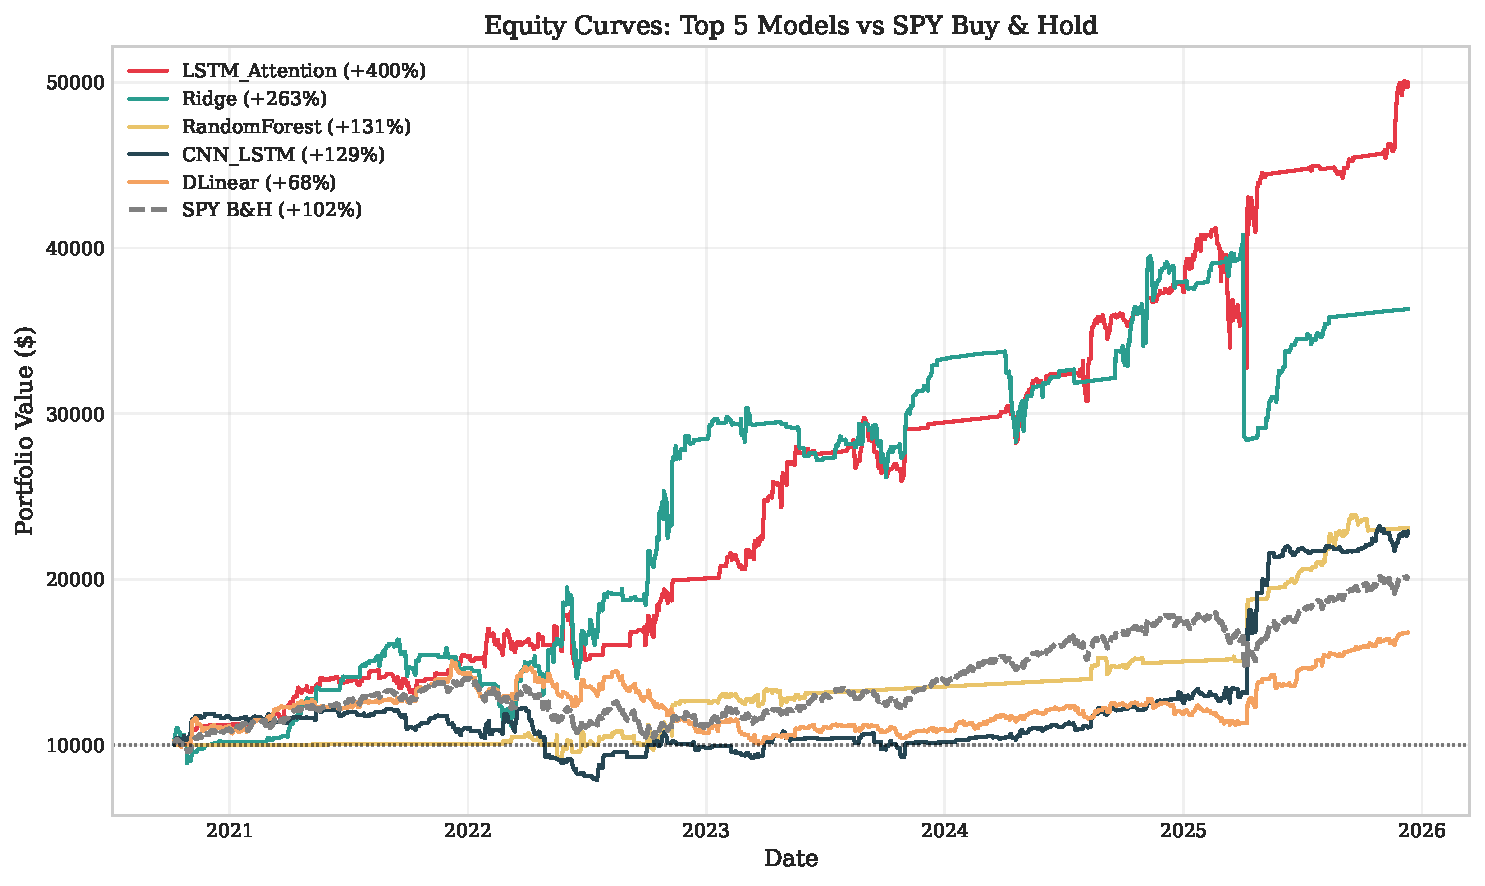
\includegraphics[width=\textwidth]{figures/equity_curves_top5.pdf}
\caption{Curvas de \textit{equity} de los cinco mejores modelos vs SPY Buy \& Hold (oct. 2020 a dic. 2025, capital inicial \$10,000).}
\label{fig:equity_curves}
\end{figure}

La Figura~\ref{fig:equity_curves} muestra patrones diferenciados entre los modelos l\'ideres. El modelo LSTM+Attention presenta la trayectoria m\'as estable del grupo, con retrocesos contenidos durante los episodios de estr\'es, alcanzando un \textit{drawdown} m\'aximo del 20.5\%. Ridge ocupa la segunda posici\'on con buena estabilidad, seguido por RandomForest (15.0\% de \textit{drawdown}, el menor del grupo) y CNN-LSTM. Los cuatro modelos finalizan el per\'iodo por encima del SPY, si bien su posici\'on relativa var\'ia a lo largo del trayecto y las diferencias se consolidan sobre todo hacia el tramo final.

Detr\'as de esas trayectorias hay distribuciones de posiciones notablemente distintas entre modelos, como muestra la Tabla~\ref{tab:position_distribution}. LSTM+Attention distribuye su tiempo entre UPRO (12.2\%), SPY (32.7\%) y efectivo (55.1\%), lo que refleja una estrategia selectiva que combina exposici\'on apalancada en momentos de alta convicci\'on con posiciones moderadas cuando la se\~nal es menos intensa. En contraste, modelos como ExponentialSmoothing mantienen exposici\'on casi permanente (72\% del tiempo), mientras que AutoARIMA permanece 100\% en efectivo.

Ese comportamiento selectivo se refleja tambi\'en en las estad\'isticas de operaci\'on que resume la Tabla~\ref{tab:trading_stats}. LSTM+Attention presenta un \hyperlink{glos:profit_factor}{\textit{profit factor}} de 1.52 (el m\'as alto del grupo), con ganancias promedio de +1.5\% y p\'erdidas de $-$1.2\% por \textit{trade}, lo que contribuye a la asimetr\'ia positiva visible en la Figura~\ref{fig:pnl_distribution}. RandomForest mantiene un \textit{win rate} del 52.8\% con solo 175 \textit{trades}, consistente con su posicionamiento conservador.

\subsection{Comparaci\'on con Estrategias de Referencia Alternativas}
\label{subsec:additional_benchmarks}

La Tabla~\ref{tab:benchmarks} compara los modelos ganadores contra \textit{benchmarks} alternativos. Frente a la retenci\'on pasiva de UPRO 3x (+123\%, \textit{drawdown} $-$69.0\%), LSTM+Attention registra un retorno mayor (+395\%), un \textit{drawdown} de $-$20.5\% y un Sharpe de 1.32 frente a 0.26, sugiriendo que la selecci\'on temporal de la exposici\'on apalancada genera un perfil cualitativamente diferente al de la retenci\'on pasiva del ETF 3x. Los cuatro modelos finalizan asimismo por encima del portafolio 60/40 (+71\%) y del SPY en retorno total acumulado.
